\chapter{Contexte général du projet}
\label{chap:premierchapitre}

\begin{fquote}ce chapitre introductif est dans le but de mettre le travail dans son contexte général.
	Nous commençons tout d’abord par une présentation de l’entreprise d’accueil. Ensuite, nous
	mettons l’accent à décrire le sujet autour du quel se déroule notre projet de fin d’études. Enfin,
	nous allons faire la critique du système actuel et de proposer les solutions adéquats avant de
	mettre à disposition le langage et la méthodologie de conception.
 \end{fquote}

\clearpage
\section{Présentation de l’organisme d’accueil}

\subsection{Cadre général de travail}

\begin{figure}[hbt!]
  \centering
  
\includegraphics[width=5cm]{sqli_logo}
  \caption{Logo de la société N3RD.}
  \label{fig:logo-sqli}
\end{figure}
N3RD Créée en 2011 est une société d’ingénierie et de développement web qui, grâce à
l’utilisation des nouvelles technologies du web, est capable aujourd’hui d’assurer les différentes
tâches. \cite{wiki:sqli}.
\smallskip
\subsection{Domaines d’activité de l'entreprise}
N3RD est une société très active dans le domaine du développement Web et mobile ( sites
et applications), elle n’utilise que les dernières technologies :
\medskip
\begin{itemize}
  \item Web 2.0 et plus.
  \smallskip
  \item  Langages de développement côté serveur : PHP5, MySQL5, CSS3, HTML5
  \smallskip
  \item  Frameworks : Symphony2, Zend, Laravel et Code Igniter
  \smallskip
  \item CMSs : Prestashop, Drupal et WordPress.
  \smallskip
    \item Animation dynamique côté client : CSS3, JavaScript, Bootstrap, Ajax et JQuery.
  \smallskip
\end{itemize}
\medskip
\subsection{Mission de l'entreprise}
\begin{itemize}
	\item  Développement de sites et applications web pour tout business. 
	\smallskip
	\item Développement des solutions web personnalisées.
	\smallskip
	\item Conseils.
	\smallskip
	\item Boutiques en ligne et e-commerce.
	\smallskip
	\item Design sur mesure.
	\smallskip
	\item Création multimédia.
	\smallskip
	\item Infogérance (hébergement, gestion d’infrastructure...).
	\smallskip
	\item Création d’outils collaboratifs.
	\smallskip
	\item Optimisation pour les plateformes mobiles.
	\smallskip
	\item Création d’applications mobiles (Android IOS).
\end{itemize}

 

\section{Étude de l'existant}
\subsection{Cadre du projet}

Nous ne pouvons pas commencer ce travail sans avoir des informations et des idées claires et précises sur l’existant. L’étude de l’existant est une phase d’analyse qui consiste à faire un diagnostic sur les points forts et faibles du projet et déterminer des objectifs du nouveau système et l’ébauche de solution. Pour ce faire, il faut étudier le système existant lui même ainsi que l’environnement dans lequel il baigne.

\medskip
     
Après observation des plusieur site web université actuel nous avons constaté qu’il ne contient que les emplois du temps et les résultats en ligne ou quelques autres informations pour les etudiants(Stages..) .

\subsection{Problématique}
La formation à plusieur université se fait actuellement de façon traditionnelle (des enseignants, des étudiants et des cours sur place), et leur site ne contient ni des supports de cours ni des séries
d’exercices et n’offre pas la possibilité de passer les examens en ligne ce qui gêne les étudiants qui travaillent et veulent poursuivre leurs études en parallèle.
Alors notre mission est de résoudre
ce problème.

\subsection{Solution proposée}
En tenant compte des différents problèmes que nous avons évoqués, nous sommes amenés à
proposer une solution qui répond aux objectifs et qui pallie aux lacunes constatées aux niveau
de processus de l’existant.

 L’idée de notre projet consiste à mettre en place une application
web qui facilite l’étude à distance qui a pour principales missions de faciliter l’apprentissage
à distance en partageant les cours et les travaux dirigés entre l’étudiant et l’enseignant et en
permettant de passer les examens et d’avoir les notes et les résultats en ligne. 
\section{Planification et conduite du projet}
\subsection{Démarche adoptée}
Dans cette section, nous dévoilons le processus simplifié que nous préconisons pour la modélisation du système.
Nous présenterons également les principes fondamentaux du EXtreme Programming (XP) et
Scrum, afin d’éclairer les idées fortes auxquelles se rattache la démarche pratique adoptée dans
la suite du rapport.
	)
\begin{table} [!ht]
	\centering
	%	\centering
	\begin{tabular} { | m{5em} | m{7cm}| m{6cm} | }\hline
		\rowcolor[gray]{0.85}
		..... & Scrum &EXtreme Programming (XP) \\  \hline
		Description      & \small (La méthode s’appuie sur le découpage d’un
		projet en «sprint»,
		ainsi que l’autoorganisation de
		l’équipe de développement.
		Chaque sprint commence par une
		estimation suivie
		d’une planification
		opérationnelle.Le
		sprint se termine par
		une démonstration de
		ce qui a été achevé, et
		contribue à augmenter
		la valeur d’affaires du
		produit.)
		& \small (Ensemble de «Best
		Practices » de développement (Idéal pour
		le travail en groupe).
		- Cible des projets
		de moins de dix personnes.    \\    \hline
		Points forts )     &-Amélioration de la
		communication.
		-Règles définies clairement.
		-Augmentation de
		productivité.
		& -Simple à mettre en
		œuvre.
		-Fait une large place
		aux aspects techniques :prototypes,
		règles de développement, tests. . .  \\    \hline
		Points faibles    &  - Violation de responsabilité.
		-L’équipe ne se prete
		pas au SCRUM.&\small (- Ne couvre pas les
		phases en amont et
		en aval au développement : capture des besoins, support, maintenance, tests d’intégration. . .
		-Assez flou dans sa
		mise en œuvre.)   \\    \hline	
		
	\end{tabular}
	\caption{ Etude comparative entre les approches agiles}\label{tab: first-table}	
\end{table}

\clearpage
\subsubsection{presentation de la methode Scrum }
Scrum : Aujourd’hui « Scrum » est la méthode agile la plus populaire. Ce terme signifie «
mêlée » au rugby. La méthode scrum s’appuie sur des « sprints » qui sont des espaces temps
assez courts pouvant aller de quelques heures jusqu’à un mois. Généralement et de préférence
un sprint s’étend sur deux semaines. À la fin de chaque sprint, l’équipe présente ce qu’elle a
ajouté au produit.
\subsubsection{Processus de développement}
La nature du projet et sa forte dépendance aux acteurs du domaine sont les raisons qui expliquent le fait d’être toujours à l’écoute du client et prêt à répondre à ses nouveaux besoins. C’est pour cela, l’équipe du projet a opté pour un cycle de développement agile et plus précisément SCRUM.

\medskip

Le principe de la méthodologie SCRUM est de développer un logiciel de manière incrémentale en maintenant une liste totalement transparente des demandes d'évolutions ou de corrections à implémenter (backlog).

\medskip

Avec des livraisons très fréquentes, toutes les 4 semaines en général, le client reçoit un logiciel à chaque itération. Plus nous avançons dans le projet, plus le logiciel est complet et possède de plus en plus de fonctionnalités.

\medskip

Pour cela, la méthode s'appuie sur des développements itératifs à un rythme constant d'une durée de 2 à 4 semaines (2 semaines pour notre cas) comme le montre la figure \ref{fig:scrum} :

\begin{figure}[ht]
  \centering
  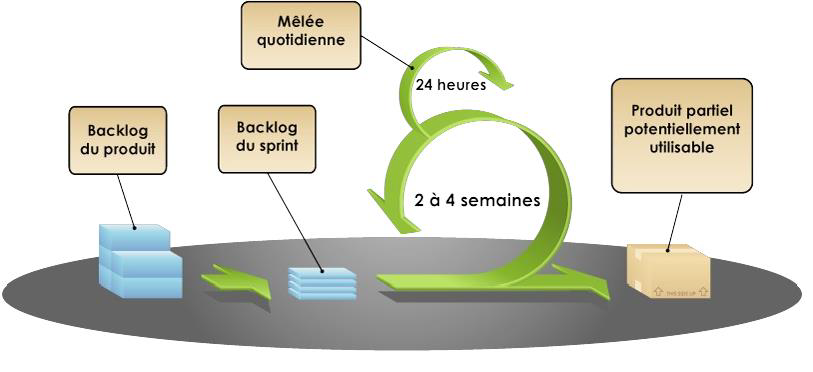
\includegraphics[width=15cm,height=6.2cm]{scrum}
  \caption{Cycle de vie de la méthodologie scrum.}
  \label{fig:scrum}
\end{figure}
\FloatBarrier

Le schéma illustre un exemple de planification en Scrum : les itérations (sprints) durent en pratique entre 2 et 4 semaines, et possède chacune un but. Le but de chaque sprint une liste d'items du backlog de produit ou de fonctionnalités à réaliser. Ces items sont décomposés par l'équipe en tâches élémentaires de quelques heures.

\medskip

Comme nous pouvons le remarquer dans cette figure, pour mettre en place la méthode SCRUM, il faut tout d'abord définir les différentes fonctionnalités de notre application qui forment le backlog du produit. Ensuite, vient l'étape de la planification du sprint pour définir le plan détaillé d'une itération.

\medskip

Durant un sprint, il y a toujours des réunions quotidiennes entre les différents collaborateurs du projet afin de présenter l'état d'avancement des différentes tâches en cours, les difficultés rencontrées ainsi que les tâches restantes à réaliser. Une fois le produit partiel est prêt, nous vérifions la conformité de ce qui a été fait durant le sprint et nous pouvons alors l'améliorer en procédant à l'étape de rétrospective.

\medskip
\subsubsection{l'equipe Scrum}
Scrum est considéré comme un cadre ou un «framework» de gestion de projet. Ce cadre est
constitué d’une définition des rôles, il s’articule autour des trois rôles qui sont principalement les suivants :

\medskip

\begin{itemize}
  \item \textbf{Product Owner} :\small ( Dans la majorité des projets, le responsable produit (product owner) est le responsable de l'équipe projet client. C'est lui qui va définir et prioriser la liste des fonctionnalités du produit et choisir la date et le contenu de chaque sprint sur la base des valeurs (charges) qui lui sont communiquées par l'équipe.)
  \smallskip
  \item \textbf{ScrumMaster} : Véritable facilitateur sur le projet, il veille à ce que chacun puisse travailler au maximum de ses capacités en éliminant les obstacles et en protégeant l'équipe des perturbations extérieures.
  \smallskip
  \item \textbf{Équipe de dévelopement} : elle regroupe l’ensemble des rôles habituellement nécessaires à un projet, à savoir le concepteur, le développeur, le testeur, etc. L'équipe s'organise elle-même et elle reste inchangée pendant toute la durée d'un sprint.

\textbf{Dans notre cas, les rôles sont répartis comme suit :}

\end{itemize}

\begin{table} [!ht]
	\centering
	\begin{tabular} {|c|c|}\hline
		Rôle & Personne \\  \hline
		Product owner     & La société N3RD      \\    \hline
		Scrum Master     & Mr Ousleti nizar    \\    \hline
		Équipe de développement    &  Mr kouki hamza ,
		Mlle khalfi khawla     \\    \hline	
		
	\end{tabular}
	\caption{Equipe Scrum}\label{tab: first-table}	
\end{table}
\clearpage
\subsubsection{les événements Scrum}
Dans le cadre du scrum, il y a 05 événements pour créer de la régularité et minimiser le besoin de rencontres. Tous les événements sont classés dans le temps (time-boxed), ce qui signifie que ces événements ont une durée maximale.
\begin{itemize}[label=$\square$,leftmargin=* ,parsep=0cm,itemsep=0cm,topsep=0cm]
	\item \textsf{Sprint:} c’est le cœur du scrum. Un sprint est lorsqu’un incrément de produit est créé. Un incrément est une partie utilisable et potentiellement fonctionnelle du produit final. Les sprints sont classés dans le temps pour un mois ou moins. Chaque sprint a un objectif de ce qui doit être construit. 
	\item \textsf{La planification du sprint (Sprint planning)} est l’événement où l’équipe scrum définit ce qui sera livré dans un sprint. Cet événement est limité dans le temps à un maximum de huit heures pour un sprint d’un mois. Dans la planification du sprint, l’équipe scrum définira ce qui peut être livré au prochain incrément et combien de travail est nécessaire pour atteindre cet objectif. L’entrée principale de cette réunion est le Product Backlog où le Product Owner et le DevTeam choisiront les éléments qui seront inclus dans ce sprint pour atteindre l’objectif du sprint. 
	\item \textsf{Le Daily scrum} est une réunion quotidienne de 15 minutes pour DevTeam où ils mettront à jour le statut de travail et les plans pour les prochaines 24 heures. Cette réunion est utilisée pour inspecter l’état d’avancement du sprint. Lors de cette réunion, chaque membre du DevTeam répondra aux questions suivantes:
	\begin{enumerate}
		\item Qu’est-ce qui a été accompli depuis la dernière réunion?
		\item Que fera-t-on avant la prochaine rencontre?
		\item Voyez-vous un obstacle qui vous empêche, ou le DevTeam, d’atteindre l’objectif de sprint?
	\end{enumerate}
	\item \textsf{La revue de sprint (Sprint review)} est utilisée par l’équipe scrum pour présenter et inspecter l’incrémentation à la fin d’un sprint. Il est limité à quatre heures pour un sprint d’un mois. Cette réunion est destinée à obtenir des commentaires et des demandes de changement du client et des parties prenantes. Seuls les éléments considérés comme « terminés (Done)» sont inclus dans la revue de sprint. 
	\item \textsf{La rétrospective Sprint (Sprint retrospective)} est un événement destiné à traiter l’amélioration. Les améliorations pourraient concerner les personnes, les relations, les processus et les outils. Il faut trois heures pour un sprint d’un mois. 
\end{itemize}

\subsection{Planning du projet}

La planification du projet est une phase importante d’avant-projet. Elle consiste à prévoir le déroulement de ce dernier tout au long des phases constituant le cycle de développement.

\medskip
\begin{itemize}
\item[$\bullet$] \textbf{Le diagramme de Gantt:}

Le diagramme de Gantt, couramment utilisé en gestion de projet, est l'un des outils les plus
efficaces pour représenter visuellement l'état d'avancement des différentes activités (tâches) qui constituent un projet.
Ce diagramme permet donc de visualiser d'un seul coup d'œil :
  \begin{itemize}
	\item[$\star$]Les différentes tâches à envisager. 
	\item[$\star$]La date de début et la date de fin de chaque tâche.
	\item[$\star$] La durée escomptée de chaque tâche. 
	\item[$\star$] Le chevauchement éventuel des tâches, et la durée de ce chevauchement.
	\item[$\star$] La date de début et la date de fin du projet dans son ensemble.
\end{itemize}





















Le diagramme de Gantt dans la figure \ref{fig:gantt} illustre le déroulement du stage dans le temps:
\end{itemize}

%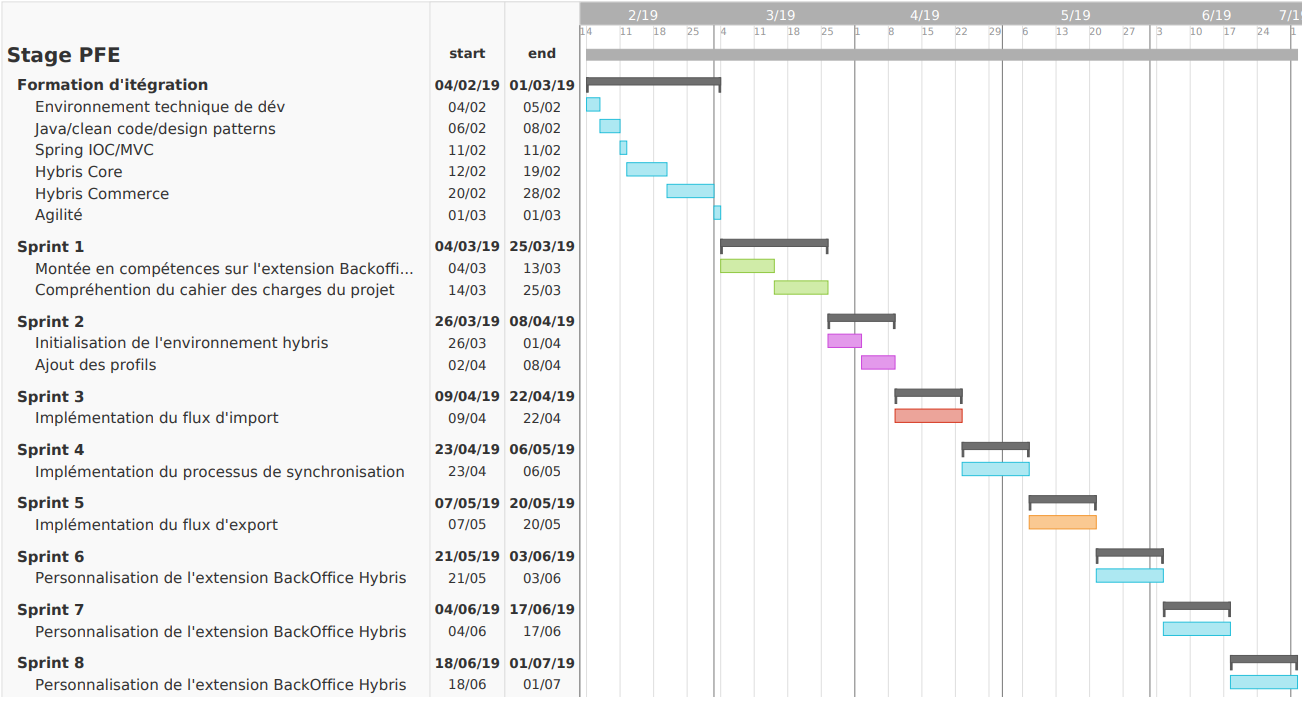
\includepdf[pages=-]{gantt.pdf}
\begin{figure}[ht]
  \centering
  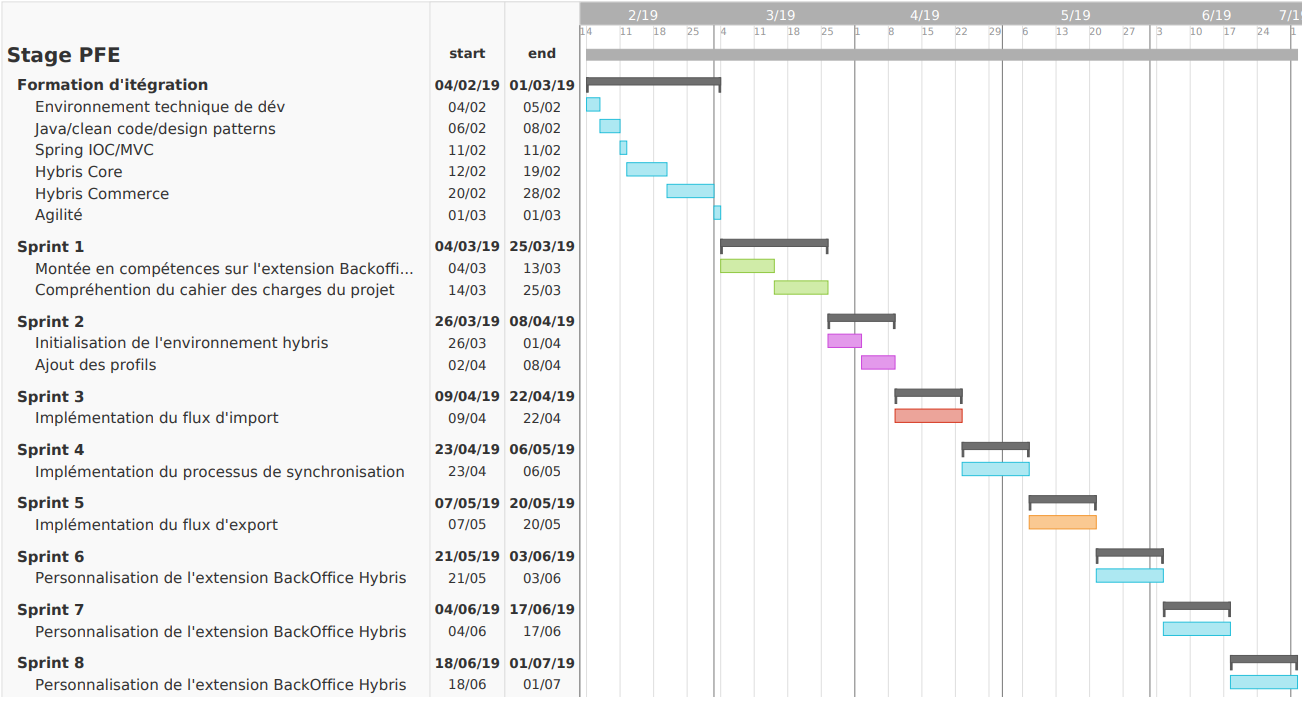
\includegraphics[height=14cm,width=16cm,angle=-90,origin=c]{gantt.PNG}
  \caption{Diagramme de gantt du projet.}
  \label{fig:gantt}
\end{figure}
\clearpage
\FloatBarrier
\subsection{La modélisation objet}
Depuis quelques années, la modélisation objet avec le langage UML est devenue une pratique
courante sur de nombreux projets informatiques. En effet, Le recours à la modélisation est
une pratique indispensable au développement logiciel, car un modèle est prévu pour arriver à
anticiper les résultats du codage.
\subsubsection{Définition de UML}
UML se définit comme un langage de modélisation graphique et textuel destiné à comprendre et décrire des besoins, spécifier et documenter des systèmes, esquisser des architectures
logicielles, concevoir des solutions et communiquer des points de vue. UML unifie à la fois les
notations et les concepts orientés objet. Il ne s’agit pas d’une simple notation graphique, car
les concepts transmis par un diagramme ont une sémantique précise.
UML s’articule autour de treize types de diagrammes, chacun d’eux étant dédié à la représentation des concepts particuliers d’un système logiciel [3].


\subsubsection{Processus de modélisation}
Le processus que nous allons présenter et appliquer tout au long de ce rapport :

\begin{itemize}
	\item Conduit par les cas d’utilisation ;
	\item Relativement léger et restreint, comme les méthodes agiles, mais sans négliger les activités
	de modélisation en analyse et conception ;
	\item Fondé sur l’utilisation d’un sous-ensemble nécessaire et suffisant du langage UML, conformément à méthodes agiles.
\end{itemize}



\section{Conclusion}

Tout au long de ce chapitre, nous avons décrit l’organisme d’accueil , nous avons aussi
formulé une petite présentation de notre projet pour vous mettre en contexte. Nous avons
ensuite fait une étude de l’existant dans l’entreprise pour pouvoir dégager les différentes lacunesainsi que les solutions envisagées. A la fin de ce chapitre, nous avons dévoilé le langage et laméthodologie de conception de notre système.
Le chapitre suivant sera consacré à la planification du projet ainsi que la spécification des
besoins
